\documentclass[letter,10pt]{article}
\usepackage[utf8]{inputenc}
\usepackage[T1]{fontenc}
\usepackage[top=1in,bottom=1in,left=1in,right=1in]{geometry}
\usepackage{amsmath,amsfonts}
\usepackage{amssymb}
\usepackage{stmaryrd}
\usepackage{graphicx}
\usepackage{url}
\usepackage{soul}
\usepackage{multirow}
\usepackage{hyperref}
\usepackage{algorithm,algorithmic}

\def\R{{\mathbb{R}}}
\def\C{{\mathbb{C}}}
\def\N{{\mathbb{N}}}
\def\Z{{\mathbb{Z}}}
\def\Ra{{\mathcal{R}}}
\def\D{{\mathcal{D}}}
\def\W{{\mathcal{W}}}
\def\SS{{\mathcal{S}}}
\def\F{{\mathcal{F}}}
\def\x{{\mathbf{x}}}
\def\CC{{\mathcal{C}}}
\def\Div{\textup{div\,}}
\def\prox{\textup{prox\,}}
\def\sign{\textup{sign}}
%opening
\title{Primal Dual optimization}
\author{J. Gilles}

\begin{document}

\maketitle

\section{Definitions and notations}
In this section, we recall some general definitions and properties from convex optimization and we also fix some notations which will be used throughout this document.
We first define the numerical gradient $\nabla$ and divergence $\Div$ operators such that the adjoint of $\nabla$ is given by $\nabla^*=-\Div$.
Given an image $u$ of size $M\times N$ where $u_{i,j}$ represents the pixel at coordinates $(i,j)$, we have
$$\nabla u_{i,j}=\left(\nabla u_{i,j,1},\nabla u_{i,j,2} \right),$$
where $\forall i,j \in D=\llbracket 1,\ldots,M \rrbracket \times \llbracket 1,\ldots,N \rrbracket$ (we will always use $D$ to denote the image domain),
\begin{equation}
\nabla u_{i,j,1}=
\begin{cases}
 u_{i+1,j}-u_{i,j} \qquad & \text{if} \quad i<M\\
 0 \qquad & \text{if} \quad i=M
\end{cases}
\quad\quad
\text{and}
\quad\quad
\nabla u_{i,j,2}=
\begin{cases}
 u_{i,j+1}-u_{i,j} \qquad & \text{if} \quad j<N\\
 0 \qquad & \text{if} \quad j=N
\end{cases}.
\end{equation}
The divergence is defined by, let $p=(p_1,p_2)$
\begin{equation}
\Div \; p_{i,j}=
\begin{cases}
p_{i,j,1}-p_{i-1,j,1} & \text{if} \quad 1<i<M\\
p_{i,j,1} & \text{if} \quad i=1\\
-p_{i-1,j,1} & \text{if} \quad i=M\\
\end{cases}
+
\begin{cases}
p_{i,j,2}-p_{i,j-1,2} & \text{if} \quad 1<j<N\\
p_{i,j,2} & \text{if} \quad j=1\\
-p_{i,j-1,2} & \text{if} \quad j=N\\
\end{cases}
\end{equation}
These two operators are implemented by the functions \textit{PD\_grad.m} and \textit{PD\_div.m}, respectively.\\

We now recall some tools from convex optimization. Given a functional $F(x)$ and an operator $K$, the Fenchel transform (or conjugate transform) is defined via the following relationship.
\begin{equation}\label{eq:fenchel}
\forall x\in X\quad,\quad F(Kx)=\max_{y\in Y}\langle Kx,y\rangle-F^*(y).
\end{equation}
The proximal operator associated to $F$ is defined by
$$\prox_{\gamma F}(x)=\underset{y\in Y}{\arg\min} \frac{1}{2}\|x-y\|_2^2+\gamma F(y).$$
In practice, the link between the proximal operator of $F$ and the proximal operator of $F^*$ is given by Moreau's identity:
$$x=\prox_{\gamma F^*}(x)+\gamma\prox_{\frac{1}{\gamma}F}\left(\frac{x}{\gamma}\right).$$

\section{General primal-dual problem}
Primal-dual problems are saddle points problems of the form
\begin{equation}\label{eq:pd}
\min_{x\in X}\max_{y\in Y}\langle Kx,y\rangle+G(x)-F^*(y),
\end{equation}
where $F$ and $G$ are functionals and $K$ is an operator. Using \eqref{eq:fenchel}, it is easy to see that this primal-dual problem is equivalent the primal problem
\begin{equation}\label{eq:primal}
\min_{x\in X} F(Kx)+G(x).
\end{equation}
On the other side, we can rewrite
\begin{align*}
\min_{x\in X}\max_{y\in Y}\langle Kx,y\rangle+G(x)-F^*(y)&=\max_{y\in Y}\min_{x\in X}\langle x,K^*y\rangle+G(x)-F^*(y)\\
&=\max_{y\in Y}\left(-\max_{x\in X}\left(-\left(\langle x,K^*y\rangle+G(x)\right)\right)\right)-F^*(y)\\
&=\max_{y\in Y} -G^*(-K^*y)-F^*(y).
\end{align*}
Thus the original primal-dual problem is also equivalent to the dual problem
$$\max_{y\in Y} -G^*(-K^*y)-F^*(y).$$
It has been proven that the solution of the primal-dual problem \eqref{eq:pd} can be achieve by the following algorithm
\begin{algorithm}[H]
\begin{algorithmic}
\STATE Initialization: choose $\tau,\sigma>0,\theta\in\{0,1\},x^0=\tilde{x}^0\in X,y^0\in Y$
\REPEAT 
\STATE $y^{n+1}=\prox_{\sigma F^*}(y^n+\sigma K\tilde{x}^n)$
\STATE $x^{n+1}=\prox_{\tau G}(x^n-\tau K^*y^{n+1})$
\STATE $\tilde{x}^{n+1}=x^{n+1}+\theta(x^{n+1}-x^n)$
\UNTIL{$N$ iterations or any convergence criteria}
\end{algorithmic}
\caption{Solution to general primal-dual problems}
\end{algorithm}
\noindent In the case $\theta=1$, convergence is guaranteed if $\tau\sigma\|K\|^2<1$ (where $\|K\|$ is the norm operator).

\section{Rudin-Osher-Fatemi, $TV-L^2$, algorithm}\label{sec:rof}
The Rudin-Osher-Fatemi (ROF) model consists in solving the following problem
$$\underset{f\in X}{\arg\min}\|\nabla f\|_1+\frac{\lambda}{2}\|f-g\|_2^2,$$
where $g$ is an input (noisy) image and $\lambda$ a regularization parameter. If we denote $K=\nabla$, $F(x)=\|x\|_1$ and $G(x)=\frac{\lambda}{2}\|x-g\|_2^2$ then we have a primal problem of the form \eqref{eq:primal}. Let denote $Y=X\times X$, we have
$$F^*(p)=\delta_P(p)=\begin{cases} 0\quad&\text{if}\; \|p\|_\infty\leq 1\\ +\infty &\text{otherwise}\end{cases},$$
where $p:Y\to\R$ and $$\|p\|_\infty=\max_{i,j}|p_{i,j}|,$$
where $$\forall i,j,|p_{i,j}|=\sqrt{p_{i,j,1}^2+p_{i,j,2}^2}.$$
Therefore,
$$\prox_{\sigma F^*}(y)=\underset{z\in Y}{\arg\min}\frac{1}{2}\|y-z\|_2^2+\sigma\delta_P(z).$$
Clearly $\delta_P$ removes all points outside the unit ball with respect to the $\|.\|_\infty$ thus this minimization problem corresponds to project $y$ on the unit $L^2$-ball. 
This is given by the following projector (this operator is implemented in the \textit{PD\_projl2.m} function):
$$\prox_{\sigma F^*}(y)_{i,j}=\frac{y_{i,j}}{\max(1,|y_{i,j}|)}.$$
On the other hand,
$$\prox_{\tau G}(x)=\underset{z\in X}{\arg\min}\frac{1}{2}\|x-z\|_2^2+\frac{\tau\lambda}{2}\|z-g\|_2^2.$$
By variational calculus, we get
$$-(x-z)+\tau\lambda(z-g)=0 \Leftrightarrow z=\frac{x+\tau\lambda g}{1+\tau\lambda}.$$
Therefore (this operator is implemented in the \textit{PD\_proxl2square.m} function),
$$\prox_{\tau G}(x)=\frac{x+\tau\lambda g}{1+\tau\lambda}.$$
Finally the primal-dual algorithm to solve the ROF model is given by (and is implemented in \textit{PD\_ROF})
\begin{algorithm}[H]
\begin{algorithmic}
\STATE Initialization: choose $\tau,\sigma,\lambda>0,\theta\in\{0,1\},f^0=\tilde{f}^0=g,p^0=\nabla g$
\REPEAT 
\STATE $p^{n+1}=\prox_{\sigma F^*}(p^n+\sigma \nabla\tilde{f}^n)$
\STATE $f^{n+1}=\prox_{\tau G}(f^n+\tau \Div p^{n+1})$
\STATE $\tilde{f}^{n+1}=f^{n+1}+\theta(f^{n+1}-f^n)$
\UNTIL{$N$ iterations or any convergence criteria}
\end{algorithmic}
\caption{Rudin-Osher-Fatemi algorithm.}
\end{algorithm}
An example is given in the following figure with $\theta=1,\tau=0.01,\lambda=18,N=100$, and since here $\|\nabla\|<\frac{1}{8}$, we choose $\sigma=0.01+\frac{1}{8\tau}$.
\begin{figure}[H]
\centering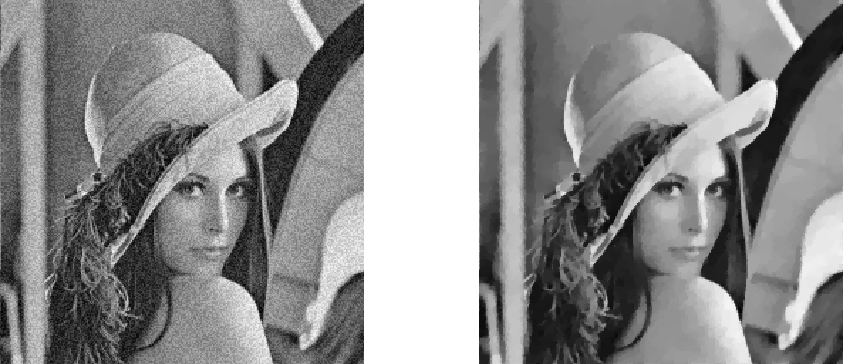
\includegraphics[width=\textwidth]{rof.png}
\caption{Result of the ROF algorithm (input on left, result on right)}
\end{figure}

\section{$TV-L^1$ algorithm}
We want to solve the model
$$\underset{f\in X}{\arg\min}\|\nabla f\|_1+\lambda\|f-g\|_1,$$
where $g$ is the input image and $\lambda$ a regularization parameter. If we denote $K=\nabla$, $F(x)=\|x\|_1$ and $G(x)=\lambda\|x-g\|_1$ then we have a primal problem of the form 
\eqref{eq:primal}. The proximal operator for $F^*$ is the same as in section~\ref{sec:rof}. We only need to find $\prox_{\tau G}$. We have
$$\prox_{\tau G}(x)=\underset{z\in X}{\arg\min}\frac{1}{2}\|x-z\|_2^2+\tau\lambda\|z-g\|_1=\underset{z\in X}{\arg\min}\|z-g\|_1+\frac{1}{2\tau\lambda}\|x-z\|_2^2.$$
If we set $w=z-g$, we get
$$\prox_{\tau G}(x)=g+\underset{w\in X}{\arg\min}\|w\|_1+\frac{1}{2\tau\lambda}\|w-(x-g)\|_2^2.$$
It known that the solution of the right hand side minimization problem is given by the shrink operator (the operations are done pixelwise, we omit the subscript $(i,j)$ to simplify the notations):
\begin{align*}
w=\sign(x-g)\max\left(|x-g|-\lambda\tau,0\right)
&=\begin{cases}
\max(x-g-\lambda\tau,0)\qquad&\text{if}\quad x-g>0\\ 
-\max(g-x-\lambda\tau,0) &\text{if}\quad x-g<0\\ 
0 &\text{if}\quad x-g=0
\end{cases}\\
&=\begin{cases}
x-g-\lambda\tau\qquad&\text{if}\quad x-g>\lambda\tau\\
0 &\text{if}\quad \lambda\tau\geq x-g>0\\
-(g-x-\lambda\tau) &\text{if}\quad x-g<-\lambda\tau\\
0 &\text{if}\quad -\lambda\tau\leq x-g<0\\
0 &\text{if}\quad x-g=0
\end{cases}\\
&=\begin{cases}
x-g-\lambda\tau\qquad&\text{if}\quad x-g>\lambda\tau\\
x-g+\lambda\tau &\text{if}\quad x-g<-\lambda\tau\\
0&\text{otherwise}
\end{cases}.
\end{align*}
Therefore (the implementation is in \textit{PD\_proxl1.m}),
$$\prox_{\tau G}(x)=g+w=
\begin{cases}
x-\lambda\tau\qquad&\text{if}\quad x-g>\lambda\tau\\
x+\lambda\tau &\text{if}\quad x-g<-\lambda\tau\\
g&\text{otherwise}
\end{cases}.$$

Finally the primal-dual algorithm to solve the TV-L1 model is given by (and is implemented in \textit{PD\_TVL1})
\begin{algorithm}[H]
\begin{algorithmic}
\STATE Initialization: choose $\tau,\sigma,\lambda>0,\theta\in\{0,1\},f^0=\tilde{f}^0=g,p^0=\nabla g$
\REPEAT 
\STATE $p^{n+1}=\prox_{\sigma F^*}(p^n+\sigma \nabla\tilde{f}^n)$
\STATE $f^{n+1}=\prox_{\tau G}(f^n+\tau \Div p^{n+1})$
\STATE $\tilde{f}^{n+1}=f^{n+1}+\theta(f^{n+1}-f^n)$
\UNTIL{$N$ iterations or any convergence criteria}
\end{algorithmic}
\caption{$TV-L^1$ algorithm.}
\end{algorithm}
An example is given in the following figure with $\theta=1,\tau=0.01,\lambda=1.5,N=100$, and since here $\|\nabla\|<\frac{1}{8}$, we choose $\sigma=0.01+\frac{1}{8\tau}$.
\begin{figure}[H]
\centering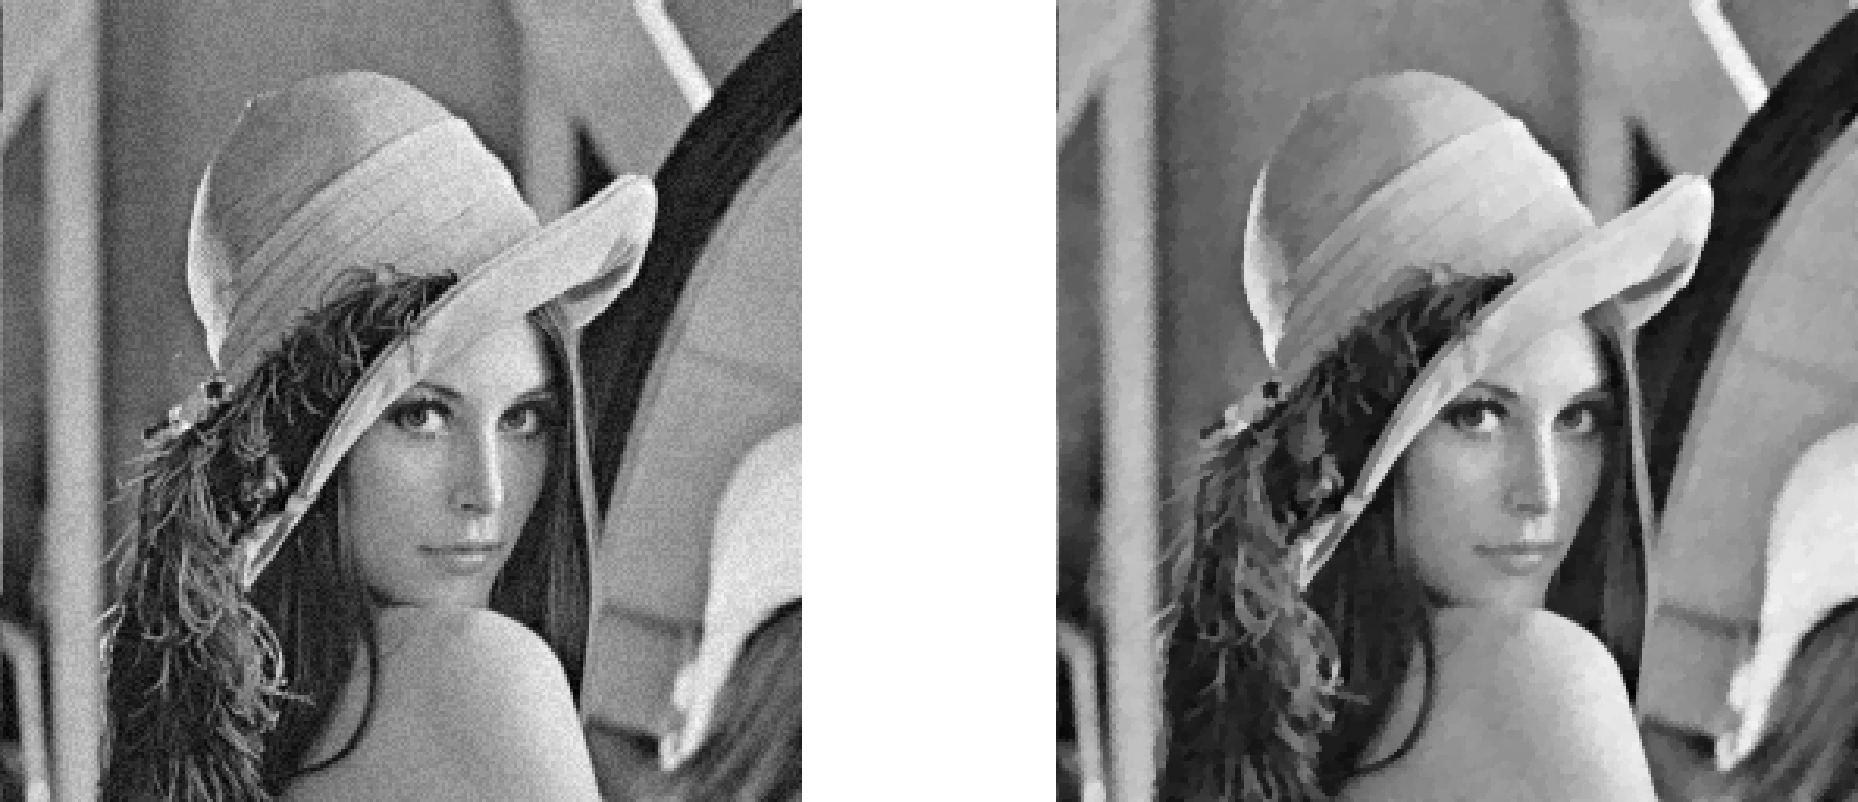
\includegraphics[width=\textwidth]{tvl1.png}
\caption{Result of the $TV-L^1$ algorithm (input on left, result on right)}
\end{figure}

\section{$TV-L^2$ inpainting}
The inpainting problem corresponds to the case when some pixels in the image $g$ are missing. We assume known the set, denoted $I$, of coordinates of the missing pixels. The 
$TV-L^2$ inpainting problem can formulated as
$$\underset{f\in X}{\arg\min}\|\nabla f\|_1+\frac{\lambda}{2}\sum_{(i,j)\in D\backslash I}(f_{i,j}-g_{i,j})^2,$$
where $g$ is the input image and $\lambda$ a regularization parameter (large values of $\lambda$ correspond to the inpainting problem while small values to a denoising case). If 
we denote $K=\nabla$, $F(x)=\|x\|_1$ and $G(x)=\frac{\lambda}{2}\sum_{(i,j)\in D\backslash 
I}(x_{i,j}-g_{i,j})^2$ then we have a primal problem of the form \eqref{eq:primal}. The proximal operator for $F^*$ is the same as in section~\ref{sec:rof}. We only need 
to find $\prox_{\tau G}$. We have
\begin{align*}
\prox_{\tau G}(x)&=\underset{z\in X}{\arg\min}\frac{1}{2}\|x-z\|_2^2+\frac{\lambda\tau}{2}\sum_{(i,j)\in D\backslash I}(z_{i,j}-g_{i,j})^2\\
&=\underset{z\in 
X}{\arg\min}\frac{1}{2}\sum_{(i,j)\in D}(x_{i,j}-z_{i,j})^2+\frac{\lambda\tau}{2}\sum_{(i,j)\in D\backslash I}(z_{i,j}-g_{i,j})^2
\end{align*}
Then if we decouple the problem for $(i,j)\in D\backslash I$ and $(i,j)\in I$, we get
\begin{itemize}
 \item if $(i,j)\in D\backslash I$, taking the derivative with respect to $z_{i,j}$, we get
 $$-(x_{i,j}-z_{i,j})+\lambda\tau(z_{i,j}-g_{i,j})=0$$
 $$\Leftrightarrow z_{i,j}=\frac{x_{i,j}+\lambda\tau g_{i,j}}{1+\lambda\tau}.$$
 \item if $(i,j)\in I$, again taking the derivative with respect to $z_{i,j}$, we get
 $$-(x_{i,j}-z_{i,j})=0 \Leftrightarrow z_{i,j}=x_{i,j}.$$
\end{itemize}
Therefore,
$$\prox_{\tau G}(x)_{i,j}=\begin{cases} x_{i,j} &\text{if}\quad (i,j)\in I\\ \frac{x_{i,j}+\lambda\tau g_{i,j}}{1+\lambda\tau}\qquad&\text{if}\quad (i,j)\in D\backslash 
I\end{cases}.$$
Moreover, if we denote the inpainting mask $$M_{i,j}=\begin{cases} 1\quad &\text{if}\quad (i,j)\in D\backslash I\\ 0 &\text{if}\quad (i,j)\in I\end{cases},$$
the previous expression can be rewritten as (the implementation is in \textit{PD\_proxtvl2inpainting.m})
$$\prox_{\tau G}(x)_{i,j}=\frac{x_{i,j}+\lambda\tau M_{i,j}g_{i,j}}{1+\lambda\tau M_{i,j}}.$$
Finally the primal-dual algorithm to solve the $TV-L2$ inpainting model is given by (and is implemented in \textit{PD\_TVL2inpainting})
\begin{algorithm}[H]
\begin{algorithmic}
\STATE Initialization: choose $\tau,\sigma,\lambda>0,\theta\in\{0,1\},f^0=\tilde{f}^0=g,p^0=\nabla g$
\REPEAT 
\STATE $p^{n+1}=\prox_{\sigma F^*}(p^n+\sigma \nabla\tilde{f}^n)$
\STATE $f^{n+1}=\prox_{\tau G}(f^n+\tau \Div p^{n+1})$
\STATE $\tilde{f}^{n+1}=f^{n+1}+\theta(f^{n+1}-f^n)$
\UNTIL{$N$ iterations or any convergence criteria}
\end{algorithmic}
\caption{$TV-L^2$ inpainting algorithm.}
\end{algorithm}
An example is given in the following figure with $\theta=1,\tau=0.01,\lambda=10000,N=100$, and since here $\|\nabla\|<\frac{1}{8}$, we choose $\sigma=0.01+\frac{1}{8\tau}$.
\begin{figure}[H]
\centering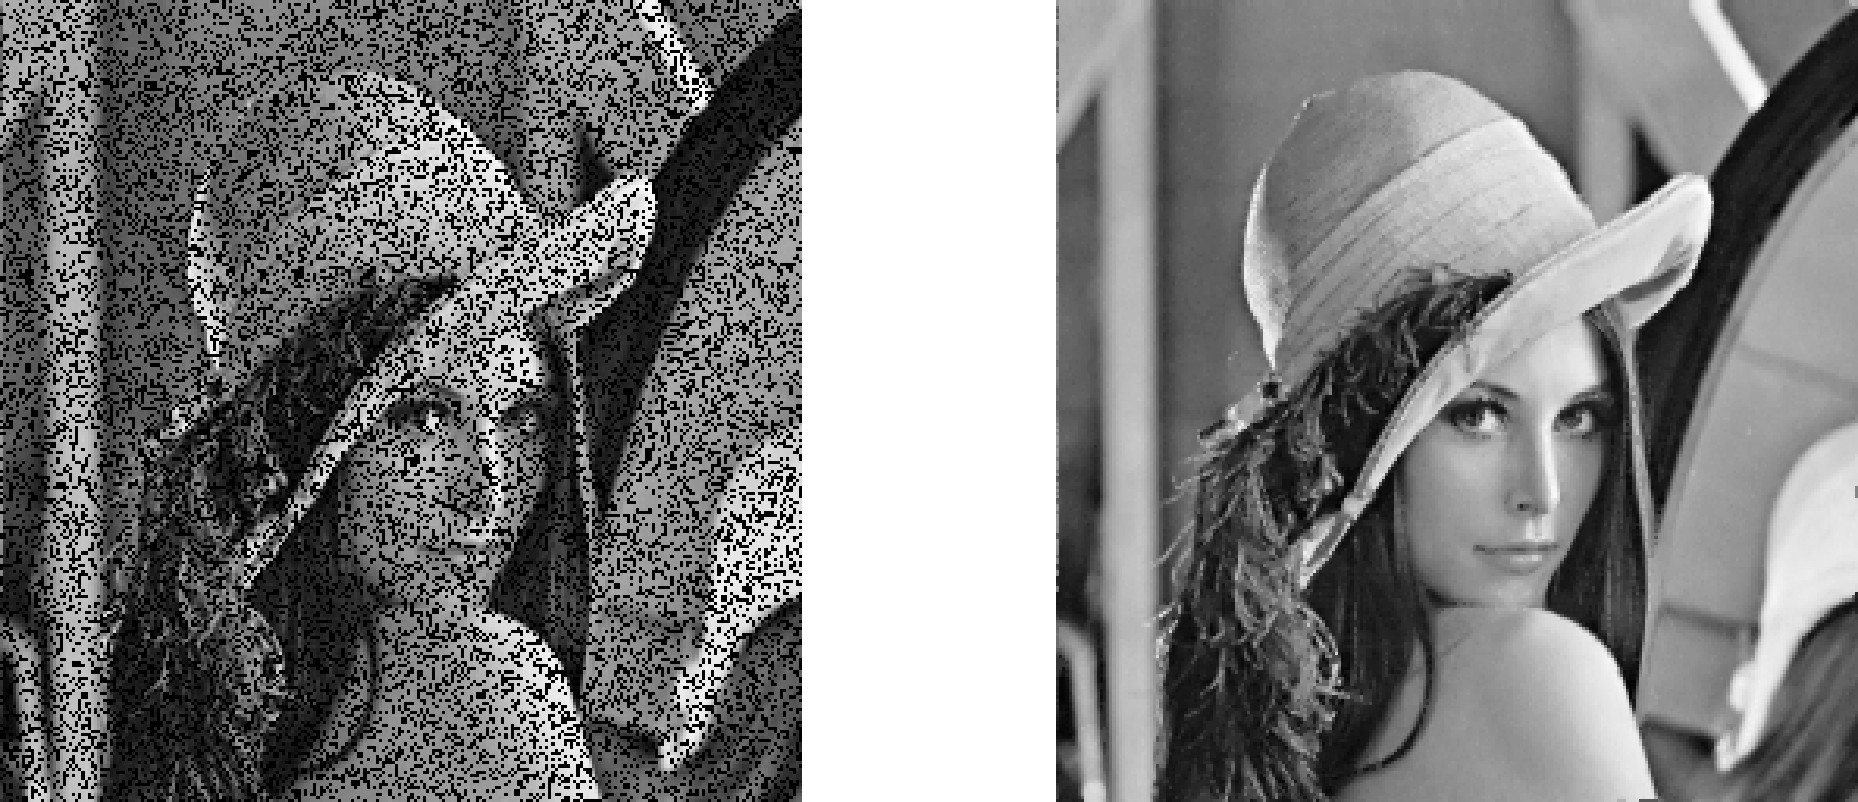
\includegraphics[width=\textwidth]{tvl2inpainting.png}
\caption{Result of the $TV-L^2$ inpainting algorithm (input on left, result on right)}
\end{figure}

\section{$TV-L^2$ multi-observations}
Here, we assume that we have a sequence of input frames $\{g_k\}_{k=1}^{N_g}$, we want solve the problem
$$\underset{f\in X}{\arg\min}\|\nabla f\|_1+\frac{\lambda}{2}\sum_{k=1}^{N_g}\|f-g_k\|_2^2.$$
If we denote $K=\nabla$, $F(x)=\|x\|_1$ and $G(x)=\frac{\lambda}{2}\sum_{k=1}^{N_g}\|x-g_k\|_2^2$ then we have a primal problem of the form \eqref{eq:primal}. The proximal 
operator 
for $F^*$ is the same as in section~\ref{sec:rof}. We only need 
to find $\prox_{\tau G}$. We have
$$\prox_{\tau G}(x)=\underset{z\in X}{\arg\min}\frac{1}{2}\|x-z\|_2^2+\frac{\lambda\tau}{2}\sum_{k=1}^{N_g}\|z-g_k\|_2^2.$$
thus
$$-(x-z)+\lambda\tau\sum_{k=1}^{N_g}(z-g_k)=0$$
$$\Leftrightarrow (1+N_g\lambda\tau)z=x+\lambda\tau\sum_{k=1}^{N_g}g_k.$$
Therefore, (the implementation is in \textit{PD\_proxtvl2multi.m})
$$\prox_{\tau G}(x)=\frac{x+\lambda\tau\sum_{k=1}^{N_g}g_k}{1+N_g\lambda\tau}.$$
Finally the primal-dual algorithm to solve the $TV-L2$ multi-observations model is given by (and is implemented in \textit{PD\_TVL2multi})
\begin{algorithm}[H]
\begin{algorithmic}
\STATE Initialization: choose $\tau,\sigma,\lambda>0,\theta\in\{0,1\},f^0=\tilde{f}^0=g_1,p^0=\nabla g_1$
\REPEAT 
\STATE $p^{n+1}=\prox_{\sigma F^*}(p^n+\sigma \nabla\tilde{f}^n)$
\STATE $f^{n+1}=\prox_{\tau G}(f^n+\tau \Div p^{n+1})$
\STATE $\tilde{f}^{n+1}=f^{n+1}+\theta(f^{n+1}-f^n)$
\UNTIL{$N$ iterations or any convergence criteria}
\end{algorithmic}
\caption{$TV-L^2$ multi-observations algorithm.}
\end{algorithm}
An example is given in the following figure with $\theta=1,\tau=0.01,\lambda=2,N=100,N_g=20$, and since here $\|\nabla\|<\frac{1}{8}$, we choose $\sigma=0.01+\frac{1}{8\tau}$.
\begin{figure}[H]
\centering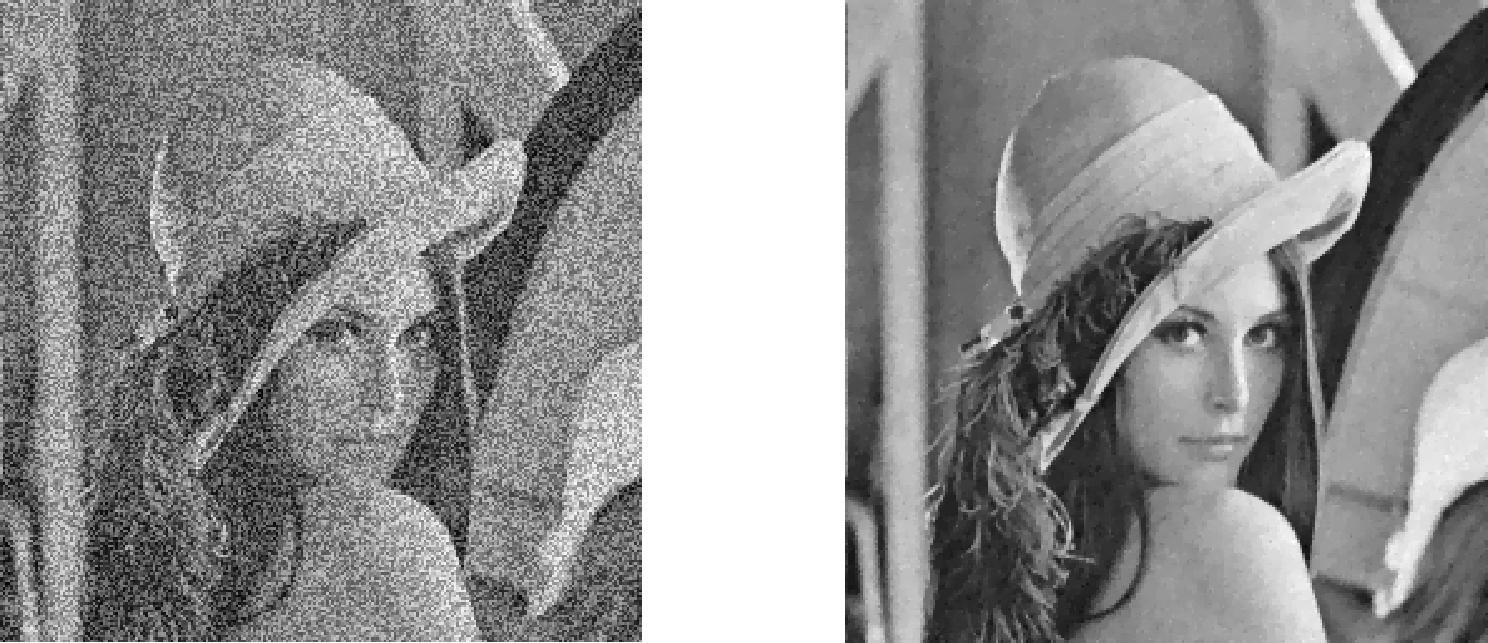
\includegraphics[width=\textwidth]{tvl2multi.png}
\caption{Result of the $TV-L^2$ multi-observations algorithm ($N_g=20$, input $g_1$ on left, result on right)}
\end{figure}

\end{document}
